\documentclass[teacher]{cours_math}
\usepackage{perso}
\usepackage{tkz-euclide}
\usetkzobj{all}
\usepackage{enumitem}
\setlist[itemize,1]{label=\textbullet}
\NewDocumentCommand{\norm}{m}{\lVert#1\rVert}
\NewDocumentCommand{\norme}{m}{\lVert\V{#1}\rVert}

\makeatletter
	\patchcmd{\tkz@DrawLine}{\begingroup}{\begingroup\makeatletter}{}{}
\makeatother

\begin{document}

\title{Orthogonalité et produit scalaire}
\level{1\iere\ S}
\chapter{12}

\maketitle


\begin{center}
  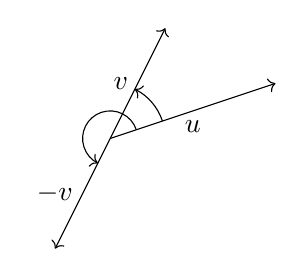
\begin{tikzpicture}[scale=.7]
    \coordinate (O) at (0,0);
    \coordinate (A) at (3,1);
    \coordinate (B) at (1,2);
    \coordinate (C) at ($-1*(B)$);
    \draw (O)node{\point};
    \draw[->] (O)--(A)node[midway,below]{$\V u$};
    \draw[->] (O)--(B)node[midway,left]{$\V v$};
    \draw[->] (O)--(C)node[midway,left]{$\bl{-\V v}$};
    \tkzMarkAngle[arrows=->](A,O,B)
    \tkzMarkAngle[size=0.5,arrows=->](A,O,C)
  \end{tikzpicture}
\end{center}
\end{document}
